\documentclass[bibliography=totoc, listof=totocnumbered]{scrartcl}
    % General document formatting
    %\usepackage[margin=0.7in]{geometry}
    %\usepackage[parfill]{parskip}
    \usepackage[utf8]{inputenc}
    %\usepackage[headsepline,footsepline]{scrpage2}
    \usepackage[onehalfspacing]{setspace}
    \usepackage{times}
    \usepackage{graphicx}
    \usepackage{fancyhdr}
    \usepackage{lastpage}
    \usepackage[affil-it]{authblk}
    \usepackage[australian,british]{babel}
    \usepackage[ddmmyyyy]{datetime}
    \usepackage[toc,page]{appendix}
    \graphicspath{ {images/} }
    \usepackage[style=numeric,sorting=none,backend=bibtex]{biblatex}
    \addbibresource{citations.bib}
    \usepackage[citecolor=black]{hyperref}

% Header and Footer Formatting-----------------------------------------------------------------------
%   Formatting of Header and Footer
% ---------------------------------------------------------------------------------------------------
%\pagestyle{scrheadings}
%\clearscrheadfoot
%\ohead{\headmark}
%\ofoot{\pagemark}

% TODO: make itemize neater

% Center all images
\makeatletter
\g@addto@macro\@floatboxreset\centering
\makeatother

\pagestyle{fancy}
\renewcommand{\dateseparator}{.}

\lhead{Technical Article}
\rhead{PSIT4}

\fancyfoot[L]{\footnotesize \today }
\fancyfoot[C]{\footnotesize Page \thepage\ of \pageref{LastPage}}


% Title Page Information-----------------------------------------------------------------------------
%   These are the informations printed on the title page of the article
% ---------------------------------------------------------------------------------------------------
\fancypagestyle{firstpage}
{
	\renewcommand{\headrulewidth}{0pt}
	\fancyhf{}
}\fancyfoot[R]{\footnotesize IT15ta\_ZH Group trckr}

\begin{document}
\begin{titlepage}
\thispagestyle{firstpage}
\centering

\includegraphics[width=0.3\textwidth]{logo}\par
\vspace{1cm}

{\scshape\LARGE Project trckr \par}
\vspace{0.3cm}

{\scshape\Large Technical Article\par}
\vspace{0.5cm}

{\scshape IT15ta\_ZH - PSIT4\par}
\vspace{0.5cm}
Ankeshian, Gabriel\\
\texttt{ankesgab@students.zhaw.ch}

\vspace{0.2cm}
Balidis, Dimitri\\
\texttt{baliddim@students.zhaw.ch}

\vspace{0.2cm}
Christen, Luca\\
\texttt{chrisluc@students.zhaw.ch}

\vspace{0.2cm}
Jossi, Savino\\
\texttt{jossisav@students.zhaw.ch}

\vspace{0.2cm}
Milenkovic, Daniel\\
\texttt{milendan@students.zhaw.ch}

\vspace{0.2cm}
Nominato, Angelica Helena Moreira Alves\\
\texttt{moreiane@students.zhaw.ch}

\vspace{0.2cm}
Pacassi Torrico, David\\
\texttt{pacasdav@students.zhaw.ch}

\vfill

% Bottom of the page
	{\large \today\par}
\end{titlepage}

% Proofreading Checklist
% * avoid passive voice
% * succinct sentences
% * use active voice
% * did I say don't use passive voice?

% Abstract----------------------------------------------------------------------
%   This is the abstract of the technical article
% ------------------------------------------------------------------------------
\begin{abstract}
  The main goal of this article is to describe the idea, goals and main
  functionalities of the web based application trckr. We developed trckr for
  % Since we want trckr to be all lowercase, we avoid using it at the start of
  % the sentence
  everyone who works on a project and needs an intuitive and simple web tool to
  accurately track their time spent on various tasks.
  % Hint: Empty line makes a paragraph which is semantically different from the
  % forced \\ newline (and much neater)

  The backend is written in Python with the help of the web application
  framework Django and the front-end with the Javascript UI framework Vue.js.
  Both technologies were new to most team members, but all members have proven
  themselves self-driven and learning these skills was ultimately a benefit to
  the outcome of the project.

  In order to compete with similar tools and web services, trckr focuses on
  performance and usability. To distinguish trckr from the competition, many
  features are planned to manage projects and tasks in a user-friendly manner.
  This will allow the user to leverage trckr to handle the ever increasing
  complexity in project management and task tracking found in large companies.
  Despite targeting large companies, trckr will remain open source and
  anyone can contribute, covering cases we might have never dreamed of.
\end{abstract}

\clearpage

\section{Introduction}
Time and task tracking are important activities in many businesses to gain
insights into the productivity of a team, requiring appropriate tools allowing
easier and more accurate time tracking. Many processes and methods have been
developed in the past to cover this need. Unfortunately most of them only
address a certain need or have been fine tuned to a specific company or team.
This not only leads to a loss of experience that could have been leveraged by
other teams but is also not generic enough to be adapted to different processes,
causing other companies to inappropriately adapt to the tool instead of the tool
adapting to the company.

\subsection{Objectives}
The goal with trckr is to develop and distribute a time tracking web application
that is easy to both understand and use. The most important non-functional
requirement is to focus on a small amount of steps for users to track the
important measurements. Only this will keep the user engaged and increase the
accuracy of the provided data.

\subsection{Main Features}
The user is able to:
\begin{itemize}
    \item register and log in to trckr
    \item create and edit projects
    \item create, track and edit tasks
    \item visit trckr on any device
\end{itemize}

\section{Architecture}
The trckr architecture consists of two separate applications. The business and
data layer are handled by the back-end application, while the presentation layer
is implemented through the front-end application. The back-end provides a
RESTful API, which is used by the front-end application to read and write the
necessary data.

This separation of concerns, achieved by decoupling the front-end and back-end,
allows for easy extensibility and fast development cycles. Additionally, one
back-end is able to serve multiple client applications, without any further work
required.

\section{Technologies}
\subsection{Django}
Django is an open source web framework written in Python.\cite{django} It
encourages fast, clean and simple development of web applications. One of the
main advantages is its fast setup, enabling developers to create applications
swiftly through it's Model-View-Presenter scheme. Django also comes with support
for various databases. Many users compare Django to Ruby On Rails but written in
Python. Django also follows the DRY principle (Don't Repeat Yourself).

\subsection{PostgreSQL}
PostgreSQL is an open source object-relational database.\cite{postgre} The
database is used to store all the data for trckr. PostgreSQL is fully supported
by Django and requires minimal configuration. The communication between the web
application and the database is done through Django's model layer.

\subsection{Docker}
Docker is a containerization platform, which adds an abstraction layer between
the application environment and the underlying server
infrastructure.\cite{docker} This means that the whole back-end environment can
be set up inside multiple docker containers which can be run locally as well as
on the production server.

\subsection{Node.js}
Node.js is a Javascript runtime which brings Javascript to the server
environment.\cite{nodejs} It uses an event-driven and non-blocking I/O model for
maximum efficiency while staying lightweight. This makes node.js the ideal
technology to implement the server side of the trckr front-end application.

\subsection{Vue.js}
Vue.js is a progressive framework used to build user interfaces.\cite{vuejs} It
is preferred for its simplicity and the rather shallow learning curve it
provides to new developers. The features of Vue.js allow the creation of data
structures that can be easily displayed on a website. This and the ability to
easily make calls to the back-end make it a good fit for trckr.

\subsection{CircleCI}
CircleCI is a continuous integration and deployment platform, enabling teams to
build software quickly and safely. Every time new code is committed, it runs a
test suite to confirm that the new code is functional and then immediately
deploys this new version. Thus enabling features to be created quickly, without
long and complicated deployments where certain bugs are discovered when the
product should be going live. This technology enabled the trckr developers to
implement features and immediately use them, motivating everybody to constantly
improve the product in small steps and see and feel the results immediately.

\section{Results}
The architecture was kept fairly simple, while still providing a clear
separation of concerns as illustrated in figure \ref{fig:architecture} using
Django with PostgreSQL in the back-end and the front-end based around Vue.js.

\begin{figure}[h]
    \includegraphics[width=8cm]{architecture}
    \caption{Architecture of trckr}
    \label{fig:architecture}
\end{figure}

\subsection{API}
The back-end of the trckr application implements a RESTful API using the Django
REST framework. The API provides basic CRUD operations for all the entities
available in the database. There are five main endpoints to retrieve and save
data on the server: authentication, user, projects, tasks and time entries.
Except for the authentication and user endpoints, all endpoints need an
authentication token to be accessed.

\subsubsection{Endpoints}
\begin{description}
\item[authentication] allows users to retrieve an authentication token from the
  server to access the other parts of the API. Via this endpoint, one can also
  invalidate the token.
\item[user] is only used to create new user accounts.
\item[projects] allows users create, read, update and delete projects and
  display all the tasks associated with a project.
\item[task] is used to create, read and update tasks for a given project. There
  is also a way to list all relevant time entries for a task.
\item[time entries] are also used to create, read, update and delete operations
\end{description}

Each object of an entity has a unique ID. This ID can be used to retrieve
information for that specific object by providing it in the URL when calling the
server. This is necessary when updating an object via a POST request.

\subsection{User Interface}
% SJ: I removed details about the implementation (receive a token) and rewrote
% to reflect the UX

% TODO: Check figures and references for mismatches
Before logging in, users are presented with the login screen as shown in figure
\ref{fig:trckr-login}. For users who have not yet registered an account, this
can be done here by entering some basic information like username, password,
email address and first and last name (Figure \ref{fig:trckr-register}).

\begin{figure}[h]
    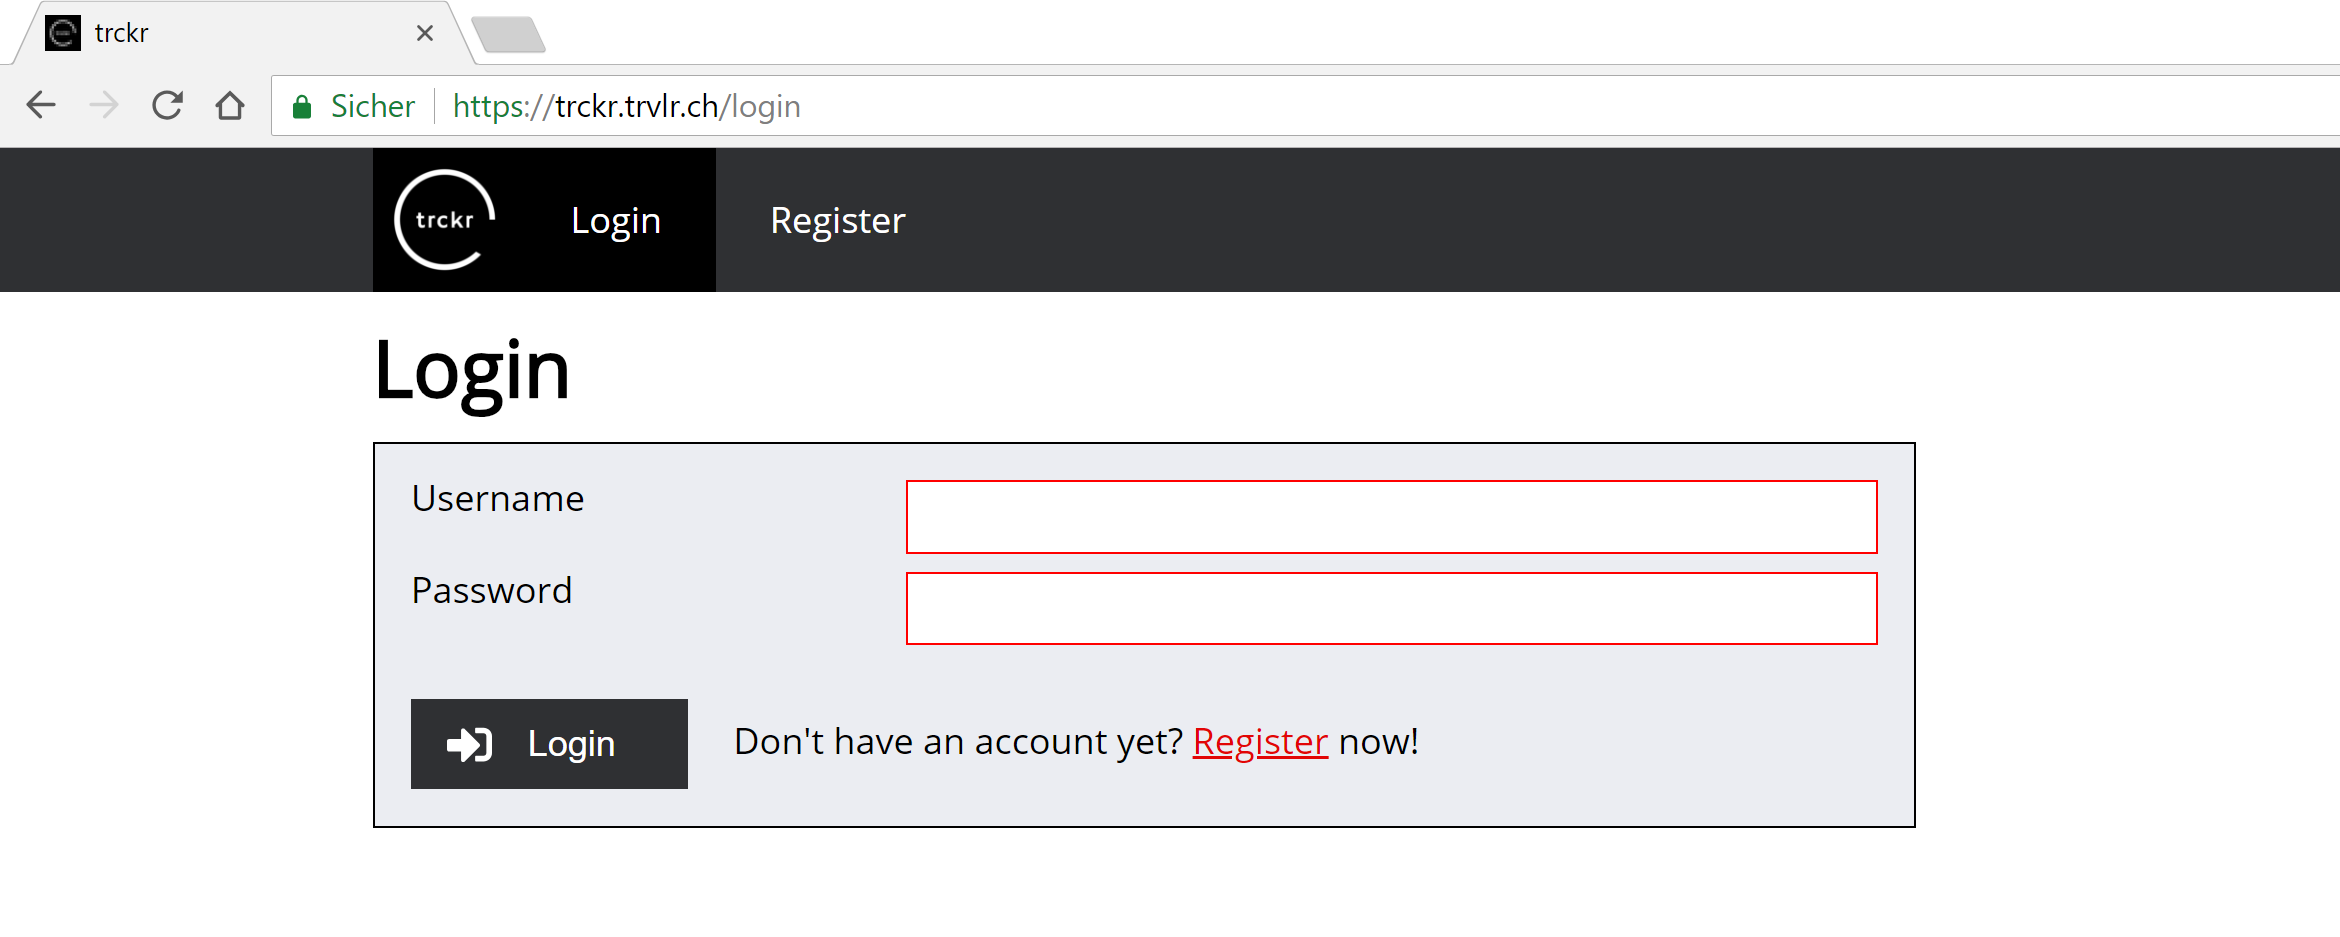
\includegraphics[width=0.8\textwidth]{trckr-login}
    \caption{The trckr login page.}
    \label{fig:trckr-login}
\end{figure}

\begin{figure}[h]
    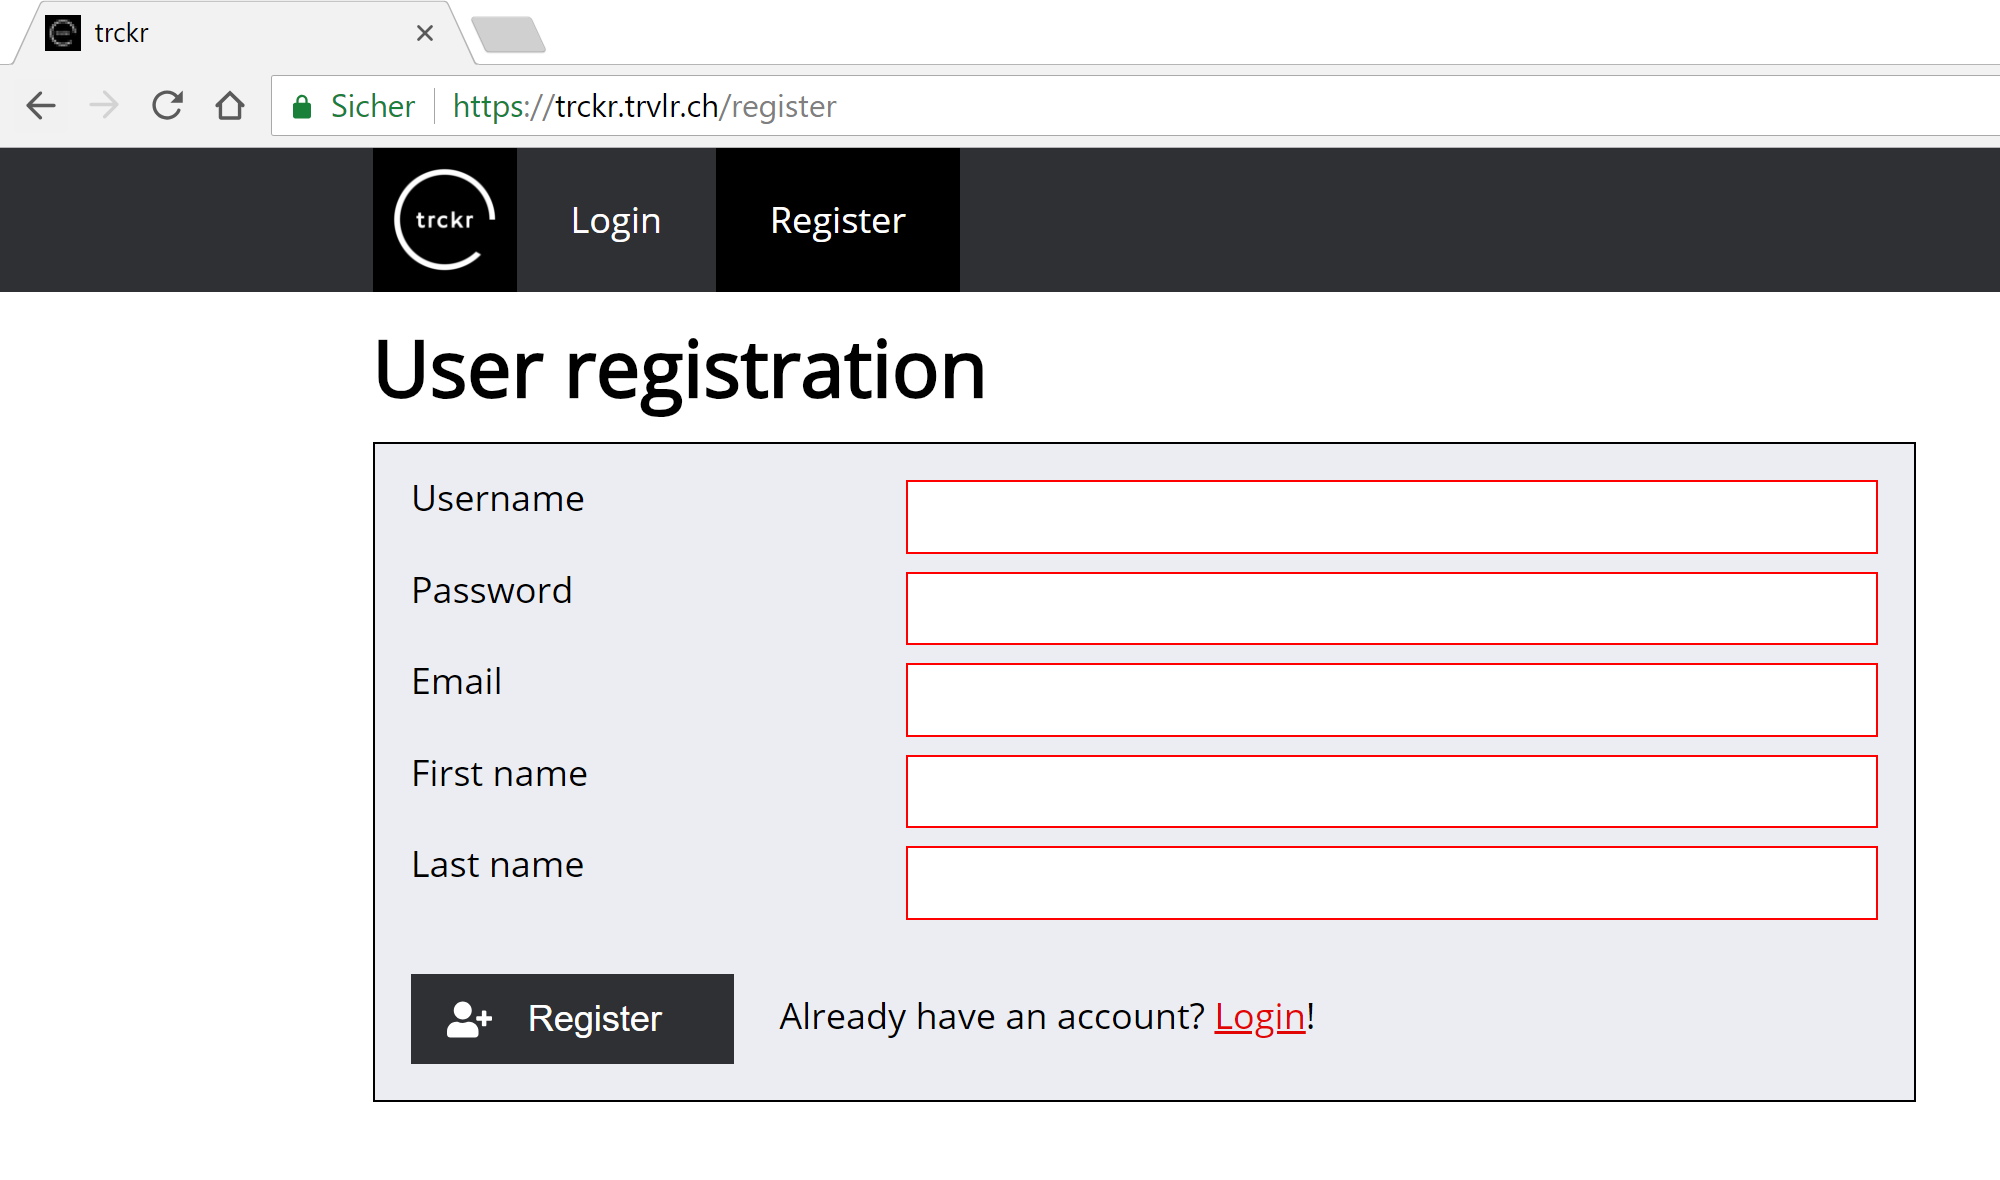
\includegraphics[width=0.8\textwidth]{trckr-register}
    \caption{The trckr registration page.}
    \label{fig:trckr-register}
\end{figure}

Once the registration process has been completed, the user can log in at the
login page. Once the user is logged in, the navigation bar at the top of the
interface will contain links to the dashboard, the projects page and the time
entries page as well as a logout button. The dashboard displays different graphs
to provide the user with a visual overview over their recent activities. This
way the user can easily see, how much time was already tracked for each task and
it enables the user to quickly proceed with their work, whithout having to
search for a relevant task.
% TODO include figure once the dashboard is finished...

The projects page shows a table of all projects that the currently logged in
user is a part of, this can be seen in figure \ref{fig:trckr-projects-table}.
There is a search box above the projects table that allows a user to filter for
a project or a group of projects containing the given keywords. To create a new
project the user will have to navigate to the projects page and click on the
"Create project" link which will open the project creation form. % please add
figure The form asks for the name of the project and optionally allows the user
to enter an description.

Each project can be viewed in more detail when the project inside the table is
clicked, as shown in figure \ref{fig:trckr-project-page}. The project page
contains the name, the description and a table of all the tasks in the selected
project.

\begin{figure}[h]
    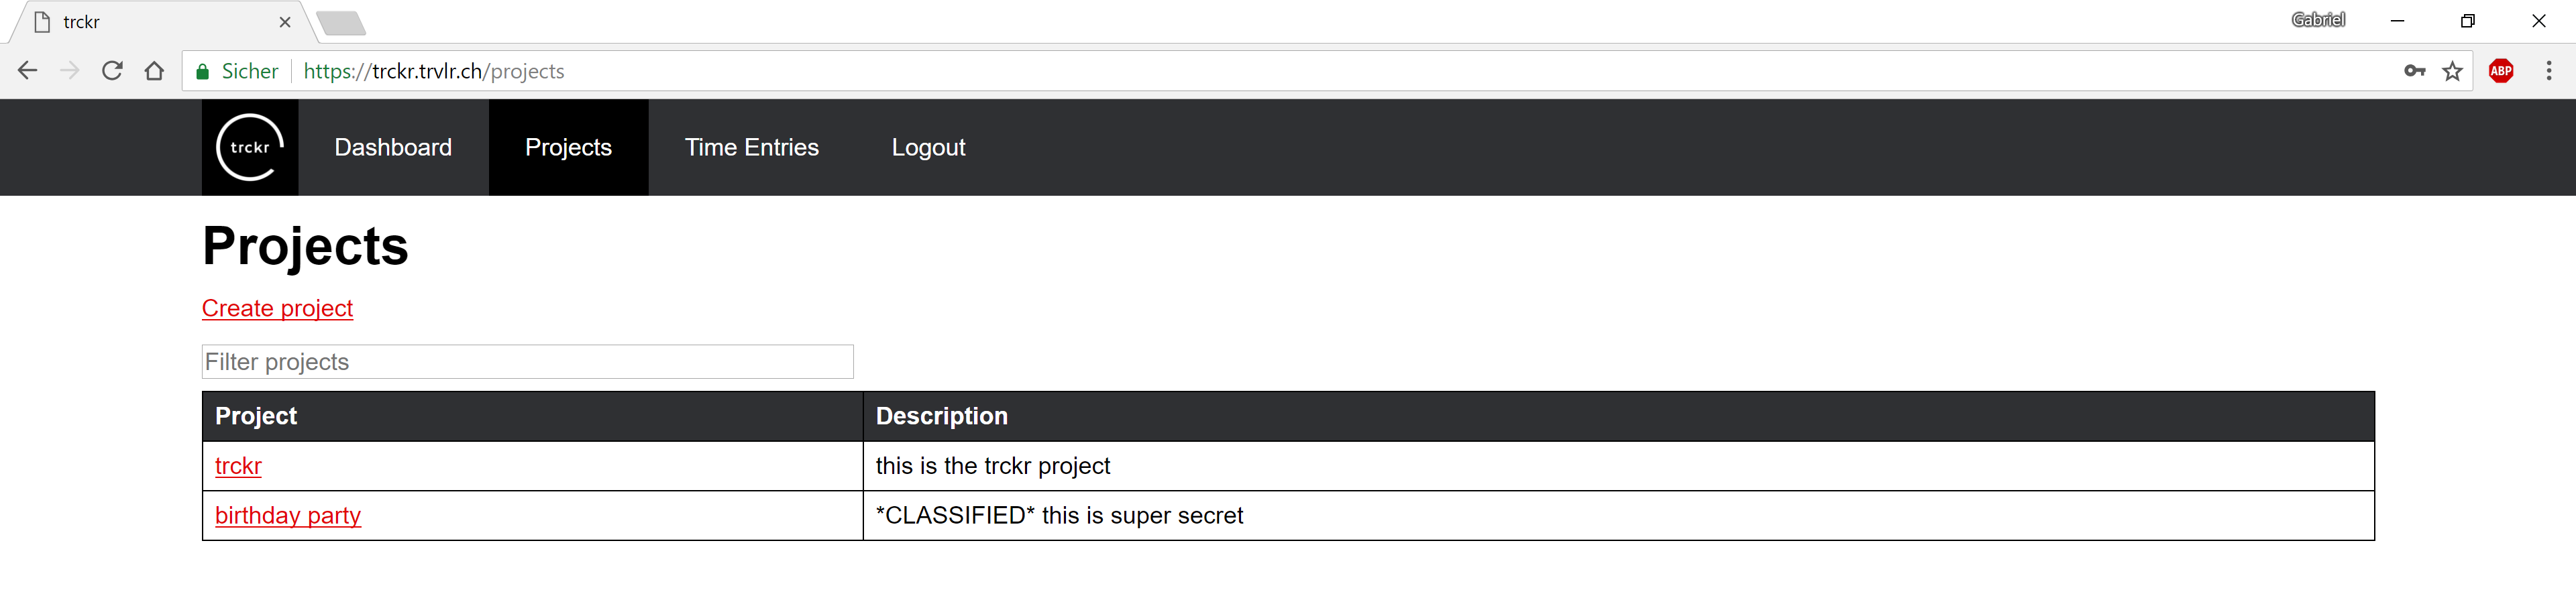
\includegraphics[width=\textwidth]{trckr-projects-table}
    \caption{The projects page with the table containing the projects.}
    \label{fig:trckr-projects-table}
\end{figure}

\begin{figure}[h]
    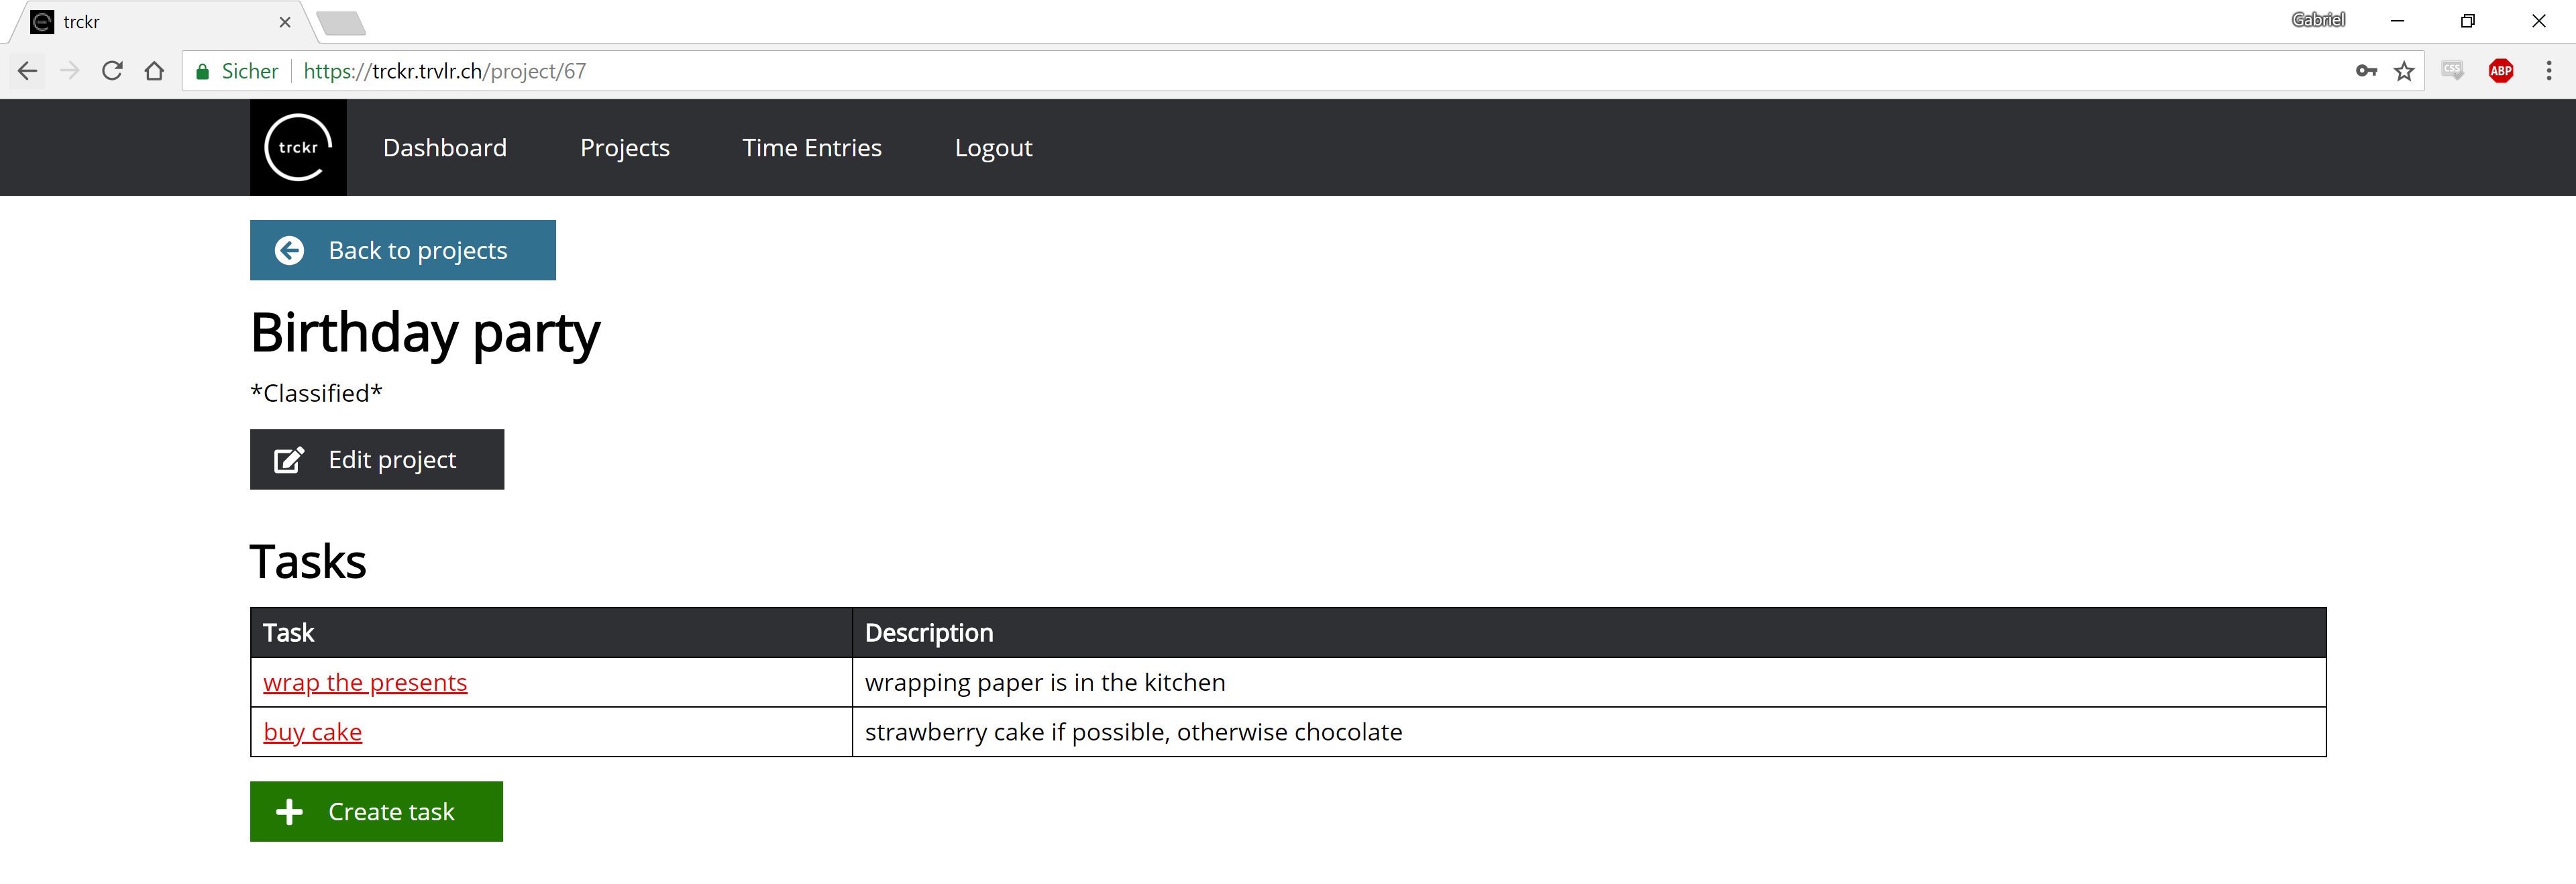
\includegraphics[width=\textwidth]{trckr-project-page}
    \caption{The project page with the table of all tasks.}
    \label{fig:trckr-project-page}
\end{figure}

Clicking on a task will display it's details like the name and description of
the task. \\
On the "Time Entries" page a user can create a time entry for a
specific task of a project with the entry form shown in figure
\ref{fig:trckr-create-time-entry}. The form asks the user to first choose a
project and then a task of the project for which the time entry should be
created.

\begin{figure}[h]
    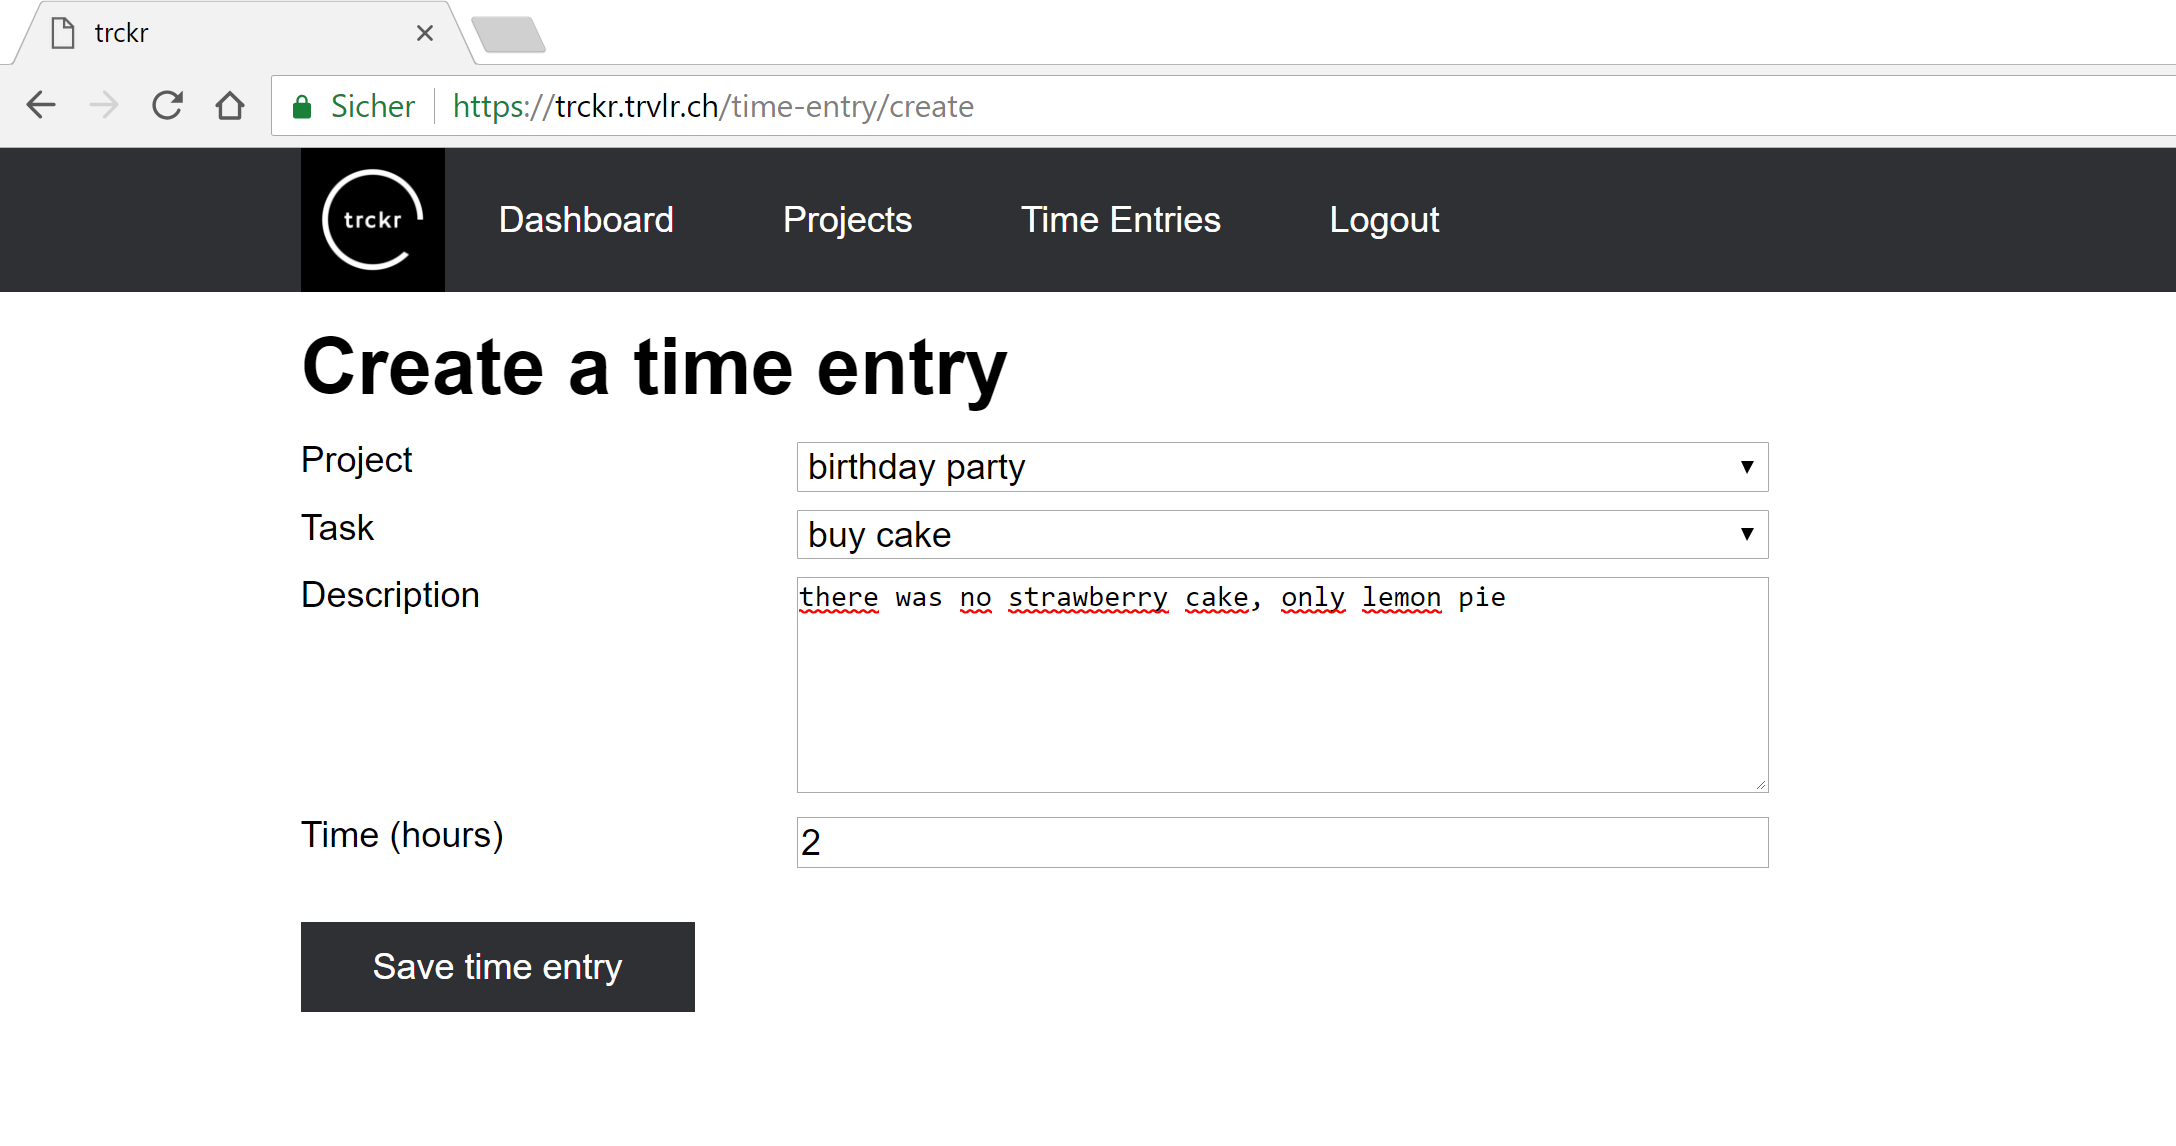
\includegraphics[width=\textwidth]{trckr-create-time-entry}
    \caption{The form to add a time entry to a task.}
    \label{fig:trckr-create-time-entry}
\end{figure}

All time entries will be displayed on the time entry page.

\section{Outlook}
By focusing on doing one thing and doing it right, it was possible to create a
modular platform. That did not just allow a clean process during development so
far, but also enables open source contributors to easily and properly add
features in the future. In the first place, the application needs some real life
usage in order to smooth the edges and fulfill the promise of being simple and
fast to use. Nevertheless, some bigger feature sets were thought up that could
not be implemented yet.

Project focused features can be improved to enable more specific project
methods, maybe even interface with ticketing or project management tools. This
enables the team leaders to gain more insight on the progress.

A desktop application could be developed to automatically track usage of certain
applications, or integrations for IDEs to track time worked on a project. By
reducing the manual intervention by the user, the tracking could become even
more accurate. This might even uncover certain inefficiencies, say by detecting
too much time waiting for tests or deployments.

\section{Conclusion}
The aim of project trckr was to create a tool, which helps people track their
time on projects. With the help of Django in the frontend and vuejs in the
frontend, we developed a webapp with modern approaches and software developing
methods. To integrate trckr into our productive environement, we used circleci,
a very useful and automated integration tool. It helped us during the
development phase target and solve bugs and other errors.

Getting started with vuejs was easy and fast for everyone, so developing single
modules for the frontend was without big effort, beside testing.

% Appendices
\clearpage
\printbibliography

\end{document}
